\documentclass{article}

\usepackage{graphicx}

\setlength{\pdfpagewidth}{8.5truein}
\setlength{\pdfpageheight}{11truein}

\def\s{\hbox{s}}
\def\m{\hbox{m}}

\usepackage{fullpage}

\addtolength{\topmargin}{-.5in}
\textheight 9in

\begin{document}

\title{Physics and Math of Music --- Day 1 --- Vibrations}
\date{Tuesday, February 5, 2002}
\author{Peter Folk ({\tt pfolk@uni}) and Paul Grayson ({\tt pgrayson@uni})}
\maketitle

\section*{Things vibrate with sine waves}
Many things, when bumped, plucked, or shaken, start vibrating back and
forth.  For example, here is a weight hanging from a string:

\begin{figure}[h]
\begin{center}
	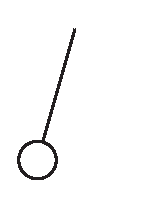
\includegraphics{figures/pendulum.pdf}
	\caption{A very simple pendulum.}
	\label{sine_wave}
\end{center}
\end{figure}

If we give it a push, it will swing back and forth for a long time.
Using a paintbrush and a long piece of paper, we can trace the motion
of the weight.  It follows a sine wave:
\begin{figure}[h]
\begin{center}
	\input figures/sine_wave.tex
	\caption{Plot of a simple sine wave: $x = A \sin(2\pi f t)$. }
	\label{sine_wave}
\end{center}
\end{figure}


\section*{Things have natural frequencies}
The pendulum swings back and forth at the same rate no
matter how hard you hit it\footnote{as long as you don't hit it {\it
too} hard!}.  For example, if it swings back and forth 10 times per
second, then $f = 4/\s$, and $f$ will be $4/\s$ even when you swing
it faster or slower.  That's why pendulums are used for making clocks
--- they keep very good time.  To calculate the natural frequency of a
pendulum, all we need to know is~$L$, its length:
$$ f = {1 \over 2\pi} \sqrt{9.8 \over L/1\m} /\s \,. $$
So, for example, if $L = 1\m$, we get
$$ f = {1 \over 2\pi} \sqrt{9.8 \over 1\m/1\m} /\s
     = {1 \over 2\pi} \sqrt{9.8 \over 1} 
     = {1 \over 2\pi} \sqrt{9.8} = 0.5/\s \,. $$
That means a one-meter pendulum takes 2 seconds to complete a full
swing.  Here's an important note: if you want to test our pendulum on
another planet, you'll have to change the~$9.8$ --- that number
represents the strength of gravity.

\section*{Things resonate}
If we give the pendulum lots of little kicks at its natural frequency,
it will start moving faster and faster.  This is called {\it
resonance}, and it occurs everywhere.  You know a lot about resonance
if you have ever used a swing: you have to pump your legs at just the
right frequency.  If you are a little bit off, the swing doesn't move
very much!

\end{document}
